\documentclass[12pt,a4paper]{article}
\usepackage[utf8]{inputenc}
\usepackage[portuguese]{babel}
\usepackage{amsmath,amssymb,amsfonts}
\usepackage{graphicx}
\usepackage{geometry}
\usepackage{booktabs}
\usepackage{listings}
\usepackage{xcolor}
\usepackage{hyperref}

\geometry{top=2.5cm, bottom=2.5cm, left=2.5cm, right=2.5cm}

\definecolor{codegreen}{rgb}{0,0.6,0}
\definecolor{codegray}{rgb}{0.5,0.5,0.5}
\definecolor{codepurple}{rgb}{0.58,0,0.82}
\definecolor{backcolour}{rgb}{0.96,0.96,0.96}

\lstdefinestyle{pythonstyle}{
    backgroundcolor=\color{backcolour},   
    commentstyle=\color{codegreen},
    keywordstyle=\color{magenta},
    numberstyle=\tiny\color{codegray},
    stringstyle=\color{codepurple},
    basicstyle=\ttfamily\footnotesize,
    breakatwhitespace=false,         
    breaklines=true,                 
    captionpos=b,                    
    keepspaces=true,                 
    numbers=left,                    
    numbersep=5pt,                  
    showspaces=false,                
    showstringspaces=false,
    showtabs=false,                  
    tabsize=4,
    literate=
        {á}{{\'{a}}}1 {à}{{\`{a}}}1 {â}{{\^{a}}}1 {ã}{{\~{a}}}1
        {é}{{\'{e}}}1 {ê}{{\^{e}}}1 {í}{{\'{i}}}1
        {ó}{{\'{o}}}1 {ô}{{\^{o}}}1 {õ}{{\~{o}}}1
        {ú}{{\'{u}}}1 {ü}{{\"{u}}}1 {ç}{{\c{c}}}1
        {Á}{{\'{A}}}1 {À}{{\`{A}}}1 {Â}{{\^{A}}}1 {Ã}{{\~{A}}}1
        {É}{{\'{E}}}1 {Ê}{{\^{E}}}1 {Í}{{\'{I}}}1
        {Ó}{{\'{O}}}1 {Ô}{{\^{O}}}1 {Õ}{{\~{O}}}1
        {Ú}{{\'{U}}}1 {Ü}{{\"{U}}}1 {Ç}{{\c{C}}}1
}
\lstset{style=pythonstyle}

\title{\textbf{Trabalho Computacional 03: Atividade 02} \\ \large Modelagem e Simulação Multifísica: Capacitor com Dois Dielétricos}
\date{}

\begin{document}

\maketitle


\section{O Problema}
O problema eletrostático consiste em determinar a distribuição de potencial $\phi(z)$ no domínio unidimensional $\Omega = [0, L]$, com $L = 1$, sujeito a uma permissividade dielétrica relativa por troços $\varepsilon_r(z)$:
\begin{equation}
    \frac{d}{dz}\left(\varepsilon_r(z)\frac{d\phi(z)}{dz}\right) = 0, \quad \forall z \in ]0, L[
\end{equation}
com condições de fronteira essenciais de Dirichlet:
\begin{equation}
    \phi(0) = V_a = 10\text{ V}, \quad \phi(L) = V_b = 0\text{ V}
\end{equation}
e a propriedade do meio definida por:
\begin{equation}
    \varepsilon_r(z) = \begin{cases} 
        3, & \text{se } 0 \le z < 0{,}5 \quad (\text{região 1}) \\ 
        1, & \text{se } 0{,}5 \le z \le 1 \quad (\text{região 2}) 
    \end{cases}
\end{equation}

\section{Solução Analítica}
Nas regiões onde a permissividade é constante, a equação diferencial reduz-se a $\frac{d^2\phi}{dz^2} = 0$, fornecendo perfis lineares:
\begin{equation}
    \phi_1(z) = A_1 z + B_1, \quad 0 \le z < 0{,}5
\end{equation}
\begin{equation}
    \phi_2(z) = A_2 z + B_2, \quad 0{,}5 \le z \le 1
\end{equation}

Aplicando as condições de contorno e de interface em $z_i = 0{,}5$:
\begin{enumerate}
    \item Condição em $z = 0$: $\phi_1(0) = 10 \implies B_1 = 10$.
    \item Condição em $z = 1$: $\phi_2(1) = 0 \implies A_2(1) + B_2 = 0 \implies B_2 = -A_2$.
    \item Continuidade do potencial em $z = 0{,}5$:
    \begin{equation}
        \phi_1(0{,}5) = \phi_2(0{,}5) \implies 0{,}5 A_1 + 10 = 0{,}5 A_2 - A_2 \implies A_1 + 20 = -A_2
    \end{equation}
    \item Continuidade do vetor deslocamento elétrico normal ($D_z = -\varepsilon_r \frac{d\phi}{dz}$):
    \begin{equation}
        3 A_1 = 1 A_2 \implies A_2 = 3 A_1
    \end{equation}
\end{enumerate}

Resolvendo o sistema de equações algébricas:
\begin{equation}
    A_1 + 20 = -3A_1 \implies 4A_1 = -20 \implies A_1 = -5, \quad A_2 = -15, \quad B_2 = 15
\end{equation}

A solução analítica exata é dada por:
\begin{equation}
    \phi(z) = \begin{cases} 
        10 - 5z, & 0 \le z \le 0{,}5 \\ 
        15(1 - z), & 0{,}5 \le z \le 1 
    \end{cases}
\end{equation}
Note-se que na interface o potencial assume o valor exato $\phi(0{,}5) = 7{,}5\text{ V}$.

\section{Dedução da Forma Fraca (FEM)}
Para contornar a descontinuidade em $\varepsilon_r(z)$, divide-se o domínio em duas integrais em torno da interface $z = 0{,}5$. Multiplicando por uma função de teste $w \in \mathcal{V} = \{ w \in H^1(\Omega) \mid w(0) = w(1) = 0 \}$:
\begin{equation}
    \int_0^{0{,}5} w \frac{d}{dz}\left(3 \frac{d\phi}{dz}\right) dz + \int_{0{,}5}^1 w \frac{d}{dz}\left(1 \frac{d\phi}{dz}\right) dz = 0
\end{equation}

Integrando cada subdomínio por partes:
\begin{align}
    \left[ 3 w \frac{d\phi}{dz} \right]_0^{0{,}5^-} - \int_0^{0{,}5} 3 \frac{dw}{dz}\frac{d\phi}{dz} dz + \left[ 1 w \frac{d\phi}{dz} \right]_{0{,}5^+}^1 - \int_{0{,}5}^1 1 \frac{dw}{dz}\frac{d\phi}{dz} dz &= 0
\end{align}

Expandindo os termos de fronteira:
\begin{align}
    3 w(0{,}5^-)\left.\frac{d\phi}{dz}\right|_{0{,}5^-} - 3 w(0)\left.\frac{d\phi}{dz}\right|_0 &+ 1 w(1)\left.\frac{d\phi}{dz}\right|_1 - 1 w(0{,}5^+)\left.\frac{d\phi}{dz}\right|_{0{,}5^+} \nonumber \\
    &- \int_0^1 \varepsilon_r(z)\frac{dw}{dz}\frac{d\phi}{dz} dz = 0
\end{align}

Como $w(0) = w(1) = 0$, $w$ é contínua na interface ($w(0{,}5^-) = w(0{,}5^+) = w(0{,}5)$), e da física tem-se que $3\left.\frac{d\phi}{dz}\right|_{0{,}5^-} = 1\left.\frac{d\phi}{dz}\right|_{0{,}5^+}$, a contribuição de interface anula-se:
\begin{equation}
    w(0{,}5) \left( 3\left.\frac{d\phi}{dz}\right|_{0{,}5^-} - 1\left.\frac{d\phi}{dz}\right|_{0{,}5^+} \right) = 0
\end{equation}

Obtém-se a forma fraca variacional:
\begin{equation}
    \int_0^1 \varepsilon_r(z) \frac{dw}{dz} \frac{d\phi}{dz} \, dz = 0, \quad \forall w \in \mathcal{V}
\end{equation}

\section{Discretização Numérica}

\subsection{Método dos Elementos Finitos (FEM)}
Adotando elementos lineares de comprimento $h$, a matriz de rigidez elementar de cada elemento $e$ é dada por:
\begin{equation}
    K^e = \frac{\varepsilon^e}{h} \begin{bmatrix} 1 & -1 \\ -1 & 1 \end{bmatrix}
\end{equation}
onde $\varepsilon^e = 3$ se o elemento estiver à esquerda de $z = 0{,}5$, e $\varepsilon^e = 1$ caso contrário. A montagem global resulta num sistema linear tridiagonal $K \Phi = F$.

\subsection{Método das Diferenças Finitas (FDM)}
Utilizando a formulação conservativa em volumes finitos centrados nos nós para lidar com o salto de condutividade dielétrica:
\begin{equation}
    \varepsilon_{i+1/2}\frac{\phi_{i+1} - \phi_i}{h} - \varepsilon_{i-1/2}\frac{\phi_i - \phi_{i-1}}{h} = 0
\end{equation}
No nó da interface $z = 0{,}5$, tem-se $\varepsilon_{i-1/2} = 3$ e $\varepsilon_{i+1/2} = 1$, conduzindo à equação discreta:
\begin{equation}
    3\phi_{i-1} - 4\phi_i + \phi_{i+1} = 0
\end{equation}
que é identicamente equivalente à linha montada no método de elementos finitos.

\section{Implementação Computacional}
O código abaixo em Python implementa as rotinas de resolução e comparação gráfica.

\begin{lstlisting}[language=Python, caption={Resolução da Atividade 02 via FEM e FDM.}]
import numpy as np
import matplotlib.pyplot as plt

# ==========================================
# ATIVIDADE 02: CAPACITOR COM DOIS DIELÉTRICOS
# ==========================================
def phi_exact(z):
    return np.where(z <= 0.5, 10.0 - 5.0 * z, 15.0 * (1.0 - z))

def solve_capacitor_fem(N_elements):
    h = 1.0 / N_elements
    z = np.linspace(0, 1, N_elements + 1)
    K = np.zeros((N_elements + 1, N_elements + 1))
    
    for e in range(N_elements):
        z_mid = (z[e] + z[e+1]) / 2.0
        eps = 3.0 if z_mid < 0.5 else 1.0
        ke = (eps / h) * np.array([[1.0, -1.0], [-1.0, 1.0]])
        K[e:e+2, e:e+2] += ke
        
    K_red = K[1:N_elements, 1:N_elements]
    F_red = - K[1:N_elements, 0] * 10.0 - K[1:N_elements, N_elements] * 0.0
    
    phi_int = np.linalg.solve(K_red, F_red)
    return z, np.concatenate(([10.0], phi_int, [0.0]))

def solve_capacitor_fdm(N_elements):
    h = 1.0 / N_elements
    z = np.linspace(0, 1, N_elements + 1)
    A = np.zeros((N_elements - 1, N_elements - 1))
    b = np.zeros(N_elements - 1)
    
    for i in range(1, N_elements):
        idx = i - 1
        z_mid_left = z[i] - h / 2.0
        z_mid_right = z[i] + h / 2.0
        eps_w = 3.0 if z_mid_left < 0.5 else 1.0
        eps_e = 3.0 if z_mid_right < 0.5 else 1.0
        
        A[idx, idx] = - (eps_w + eps_e) / (h**2)
        if idx > 0:
            A[idx, idx - 1] = eps_w / (h**2)
        if idx < N_elements - 2:
            A[idx, idx + 1] = eps_e / (h**2)
            
    b[0] -= (3.0 / (h**2)) * 10.0
    
    phi_int = np.linalg.solve(A, b)
    return z, np.concatenate(([10.0], phi_int, [0.0]))

# Execução e Apresentação dos Resultados
if __name__ == "__main__":
    z_fine = np.linspace(0, 1, 300)
    
    n_impares = [1, 3, 7, 9]

    # 1. Gráfico principal comparativo entre FEM e FDM para n = 9 (N_elements = 10)
    n_foco = 9
    N_elements_foco = n_foco + 1
    z_fem, phi_fem = solve_capacitor_fem(N_elements_foco)
    z_fdm, phi_fdm = solve_capacitor_fdm(N_elements_foco)

    plt.figure(figsize=(7, 5))
    plt.plot(z_fine, phi_exact(z_fine), 'k-', linewidth=1.5, label='Analítica')
    plt.plot(z_fem, phi_fem, 'b-s', markersize=6, label=f'FEM ($n={n_foco}$, $N_{{el}}={N_elements_foco}$)')
    plt.plot(z_fdm, phi_fdm, 'ro--', markersize=5, label=f'FDM ($n={n_foco}$, $N_{{el}}={N_elements_foco}$)')
    plt.title("Atividade 02: Potencial no Capacitor com Interface em $z=0.5$")
    plt.xlabel("z")
    plt.ylabel(r"Potencial $\phi(z)$ (V)")
    plt.legend()
    plt.grid(True)
    plt.tight_layout()
    plt.show()

    # 2. Comparação dos diferentes valores de n ímpar
    plt.figure(figsize=(8, 5))
    plt.plot(z_fine, phi_exact(z_fine), 'k-', linewidth=2, label='Analítica')
    
    marcadores = ['o--', 's--', '^--', 'd--']
    for n_val, marcador in zip(n_impares, marcadores):
        N_el = n_val + 1
        z_n, phi_n = solve_capacitor_fem(N_el)
        plt.plot(z_n, phi_n, marcador, label=f'FEM ($n={n_val}$, $N_{{el}}={N_el}$)')
        
    plt.title("Atividade 02: Comparação de Malhas com $n$ Ímpar (FEM)")
    plt.xlabel("z")
    plt.ylabel(r"Potencial $\phi(z)$ (V)")
    plt.legend()
    plt.grid(True)
    plt.tight_layout()
    plt.show()

\end{lstlisting}

\section{Resultados e Discussão da Atividade 02}

A simulação computacional foi executada variando o número de graus de liberdade internos ímpares ($n \in \{1, 3, 7, 9\}$), correspondendo a malhas de $N_{el} = n + 1$ elementos ($N_{el} \in \{2, 4, 8, 10\}$). Esta escolha garante a presença de um nó posicionado exatamente sobre a interface dos dielétricos ($z = 0{,}5$).

\subsection{Comparação entre FEM, FDM e Solução Analítica}
A Figura~\ref{fig:comparacao_metodos} apresenta o perfil de potencial $\phi(z)$ obtido para $n = 9$ ($N_{el} = 10$). Observa-se perfeita coincidência entre as aproximações por FEM, FDM e a curva de referência analítica. 

\begin{figure}[htbp]
    \centering
    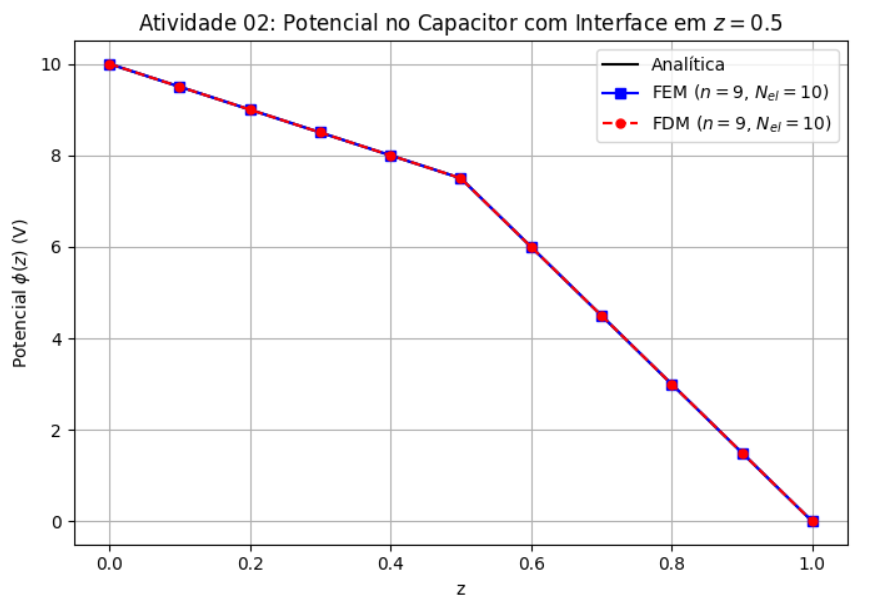
\includegraphics[width=0.72\textwidth]{image1.png}
    \caption{Distribuição do potencial eletrostático $\phi(z)$ no capacitor obtida analiticamente e numericamente via FEM e FDM ($n = 9$, $N_{el} = 10$).}
    \label{fig:comparacao_metodos}
\end{figure}

\subsection{Comportamento da Malha com $n$ Ímpar}
A Figura~\ref{fig:comparacao_malhas} ilustra as soluções fornecidas pelo método de elementos finitos com diferentes graus de refinamento espacial.

\begin{figure}[htbp]
    \centering
    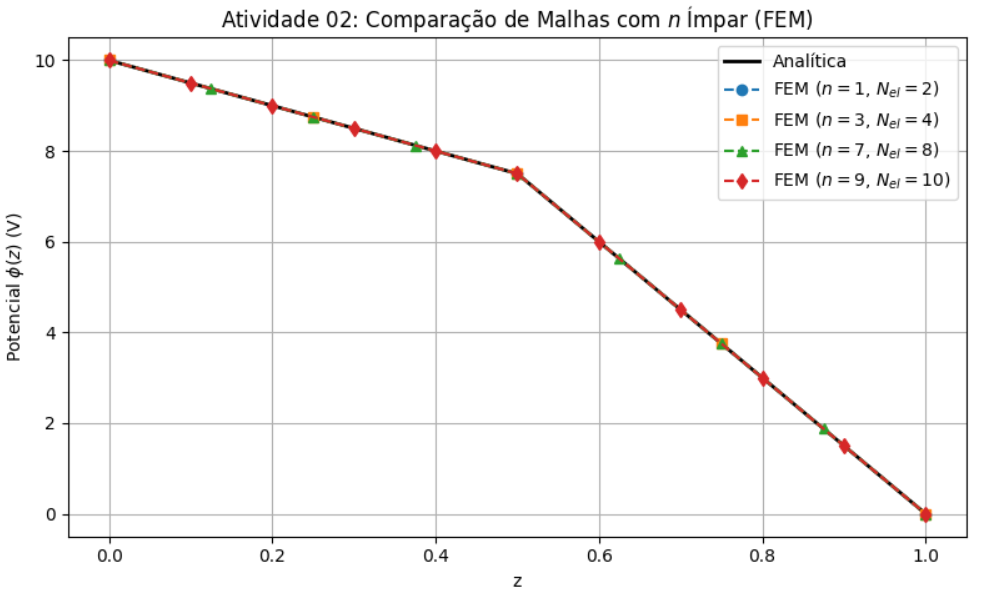
\includegraphics[width=0.72\textwidth]{image2.png}
    \caption{Comparação de malhas com diferentes ordens de $n$ ímpar via FEM contra a solução exata.}
    \label{fig:comparacao_malhas}
\end{figure}

Os valores obtidos no nó interfacial ($z = 0{,}5$) e os erros absolutos em relação ao valor analítico de $7{,}5\text{ V}$.

\noindent Como a solução exata em cada subdomínio dielétrico é de primeira ordem e os elementos utilizados possuem funções de base lineares, a projeção variacional coincide exatamente com a solução analítica nos nós da malha, independentemente do nível de refinamento adotado.

\end{document}
